% !TEX encoding = UTF-8 Unicode

\documentclass[twocolumn,10pt,a4j]{ltjsarticle}
\usepackage{kougai}

\title{VRデートアプリの提案}
\author{1932158 小池 周平  指導教員 須田 宇宙 准教授}
\date{ }

\begin{document}

\maketitle

\section{はじめに}


%背景
2015年9月に開催された「国連持続可能な開発サミット」でSDGsが掲げられた.この中に少子化も含まれており,その要因は,晩婚化の進展,交際率・婚姻率の減少\cite{naikakufu2019}などとされている.
実際に日本では,20年間で平均初婚年齢は2.6歳(男性)/3.1歳(女性)増加している.
しかし,結婚意欲は僅かに減少している程度でほぼ変化していない.
すなわち,「結婚はしたいけれど,良い相手に恵まれない」との考えが大多数を占めている\cite{naikakufu2019}.

%問題点
過去には学校や職場,友人を通じた出会いが有ったが,最近では出会いの場としてSNSを活用する者やマッチングアプリの利用者が増加している.
しかし,知らない人と2人きりで会うことに恐怖を感じたり,初デートに不安を感じるデート未経験者も少なくない\cite{prtimes,yoshimura2020}.
この問題に対して,出会ってからデートに進展するまでをサポートできれば,婚姻率上昇に繋げられるのではないかと考えた.
%この要因は「出会いの場の減少」と「交際への不安」と考えられる.
%さらに,内閣府の調査によるとデートの経験がない男性は約4割いるとされている\cite{naikakufu2022}.

%目的
そこで本研究では,2人きりで会う恐怖を緩和し,デートに対する不安を軽減するために,仮想空間内でデートする環境を構築することを目的とする.


%そこで,会う場を現実ではなく仮想空間で実施することで緊張や不安なく最初の接触を果たせるのではないかと考えた.
%これらから,本研究では少子化改善を見据えて疑似的なデートの経験を積ませ,将来的な婚姻率上昇に繋がるVRデートアプリの開発を行うことを目的とする.



%目的
\section{VRデートアプリについて}
VR空間内でデートするアプリでは個別の問題点を以下のように改善するコンセプトを考案する.
2人きりで会うことの不安については,VR空間内で擬似的にデートを行うことで改善できる.
デートの進行は,デート未経験者が失敗しないように自動進行を使用している.
全体の時間としては,40分〜1時間程度に設定している.
デート時間の前半に共通の体験をしてもらい,後半は会話する時間としてお互いの性格を知る機会を設けることとした.


\section{開発したアプリケーションについて}
図\ref{fig:screen}にVRデートアプリのプレイ画面を示す.
図中①のキャラクターは別端末から利用しているデート相手のアバターである.
自身のキャラクターと共に,仮想空間内を②の方向に自動的に進行していくというアトラクションタイプのデート体験としている.

デート体験の中でユーザーが楽しめるよう,アプリ内では早朝,朝,昼,夕方,夜が短時間で切り替わるようにしている.
アプリ内でのデートコースは1つのみであるが,時間経過を楽しめるようにしている
デートコースに目を引くような海や公園などの景色を実装しており.ユーザは自由に視点の向きを変更できることからお互いの視線を共有する事ができる.
また,会話のきっかけになるようなオブジェクトをそれぞれの景色の中に配置している.

開発したVRデートアプリケーションのシステム構造図を図\ref{fig:system}に示す.
環境を選ばずに実行できるWebアプリケーションとして開発した.
また,キャラクターの行動の同期にはWebSocketを利用している.
音声については外部の通話アプリを使用して会話をすることとした.
アプリのオブジェクトを鮮明に実装したかったが,大きな遅延が発生してしまうため低ポリゴンでの実装となった.


\begin{figure}[h]
\begin{center}
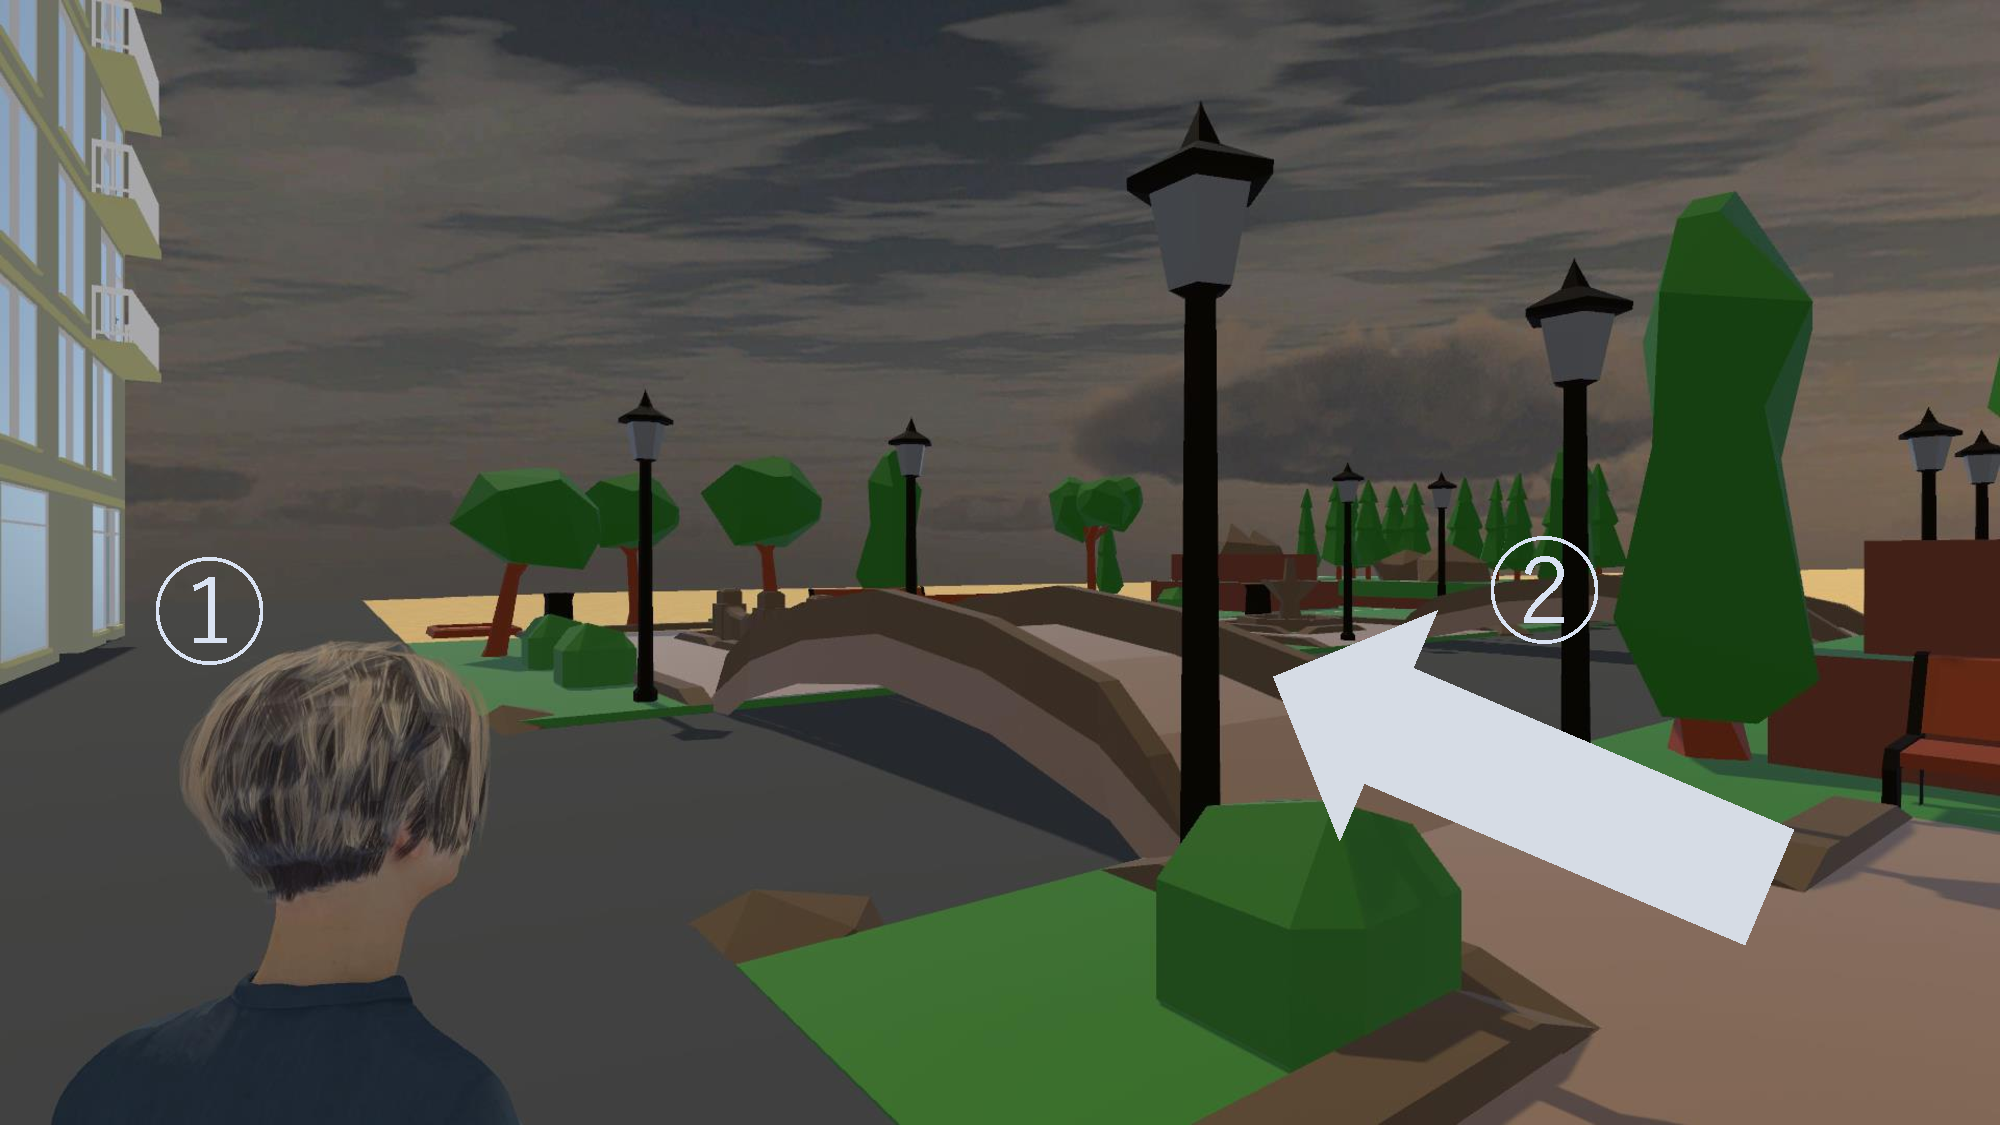
\includegraphics[width=85mm]{apurinai.pdf}
\end{center}
 \caption{VRデートアプリによるデート画面の例}
 \label{fig:screen}
\end{figure}

\begin{figure}[h]
\begin{center}
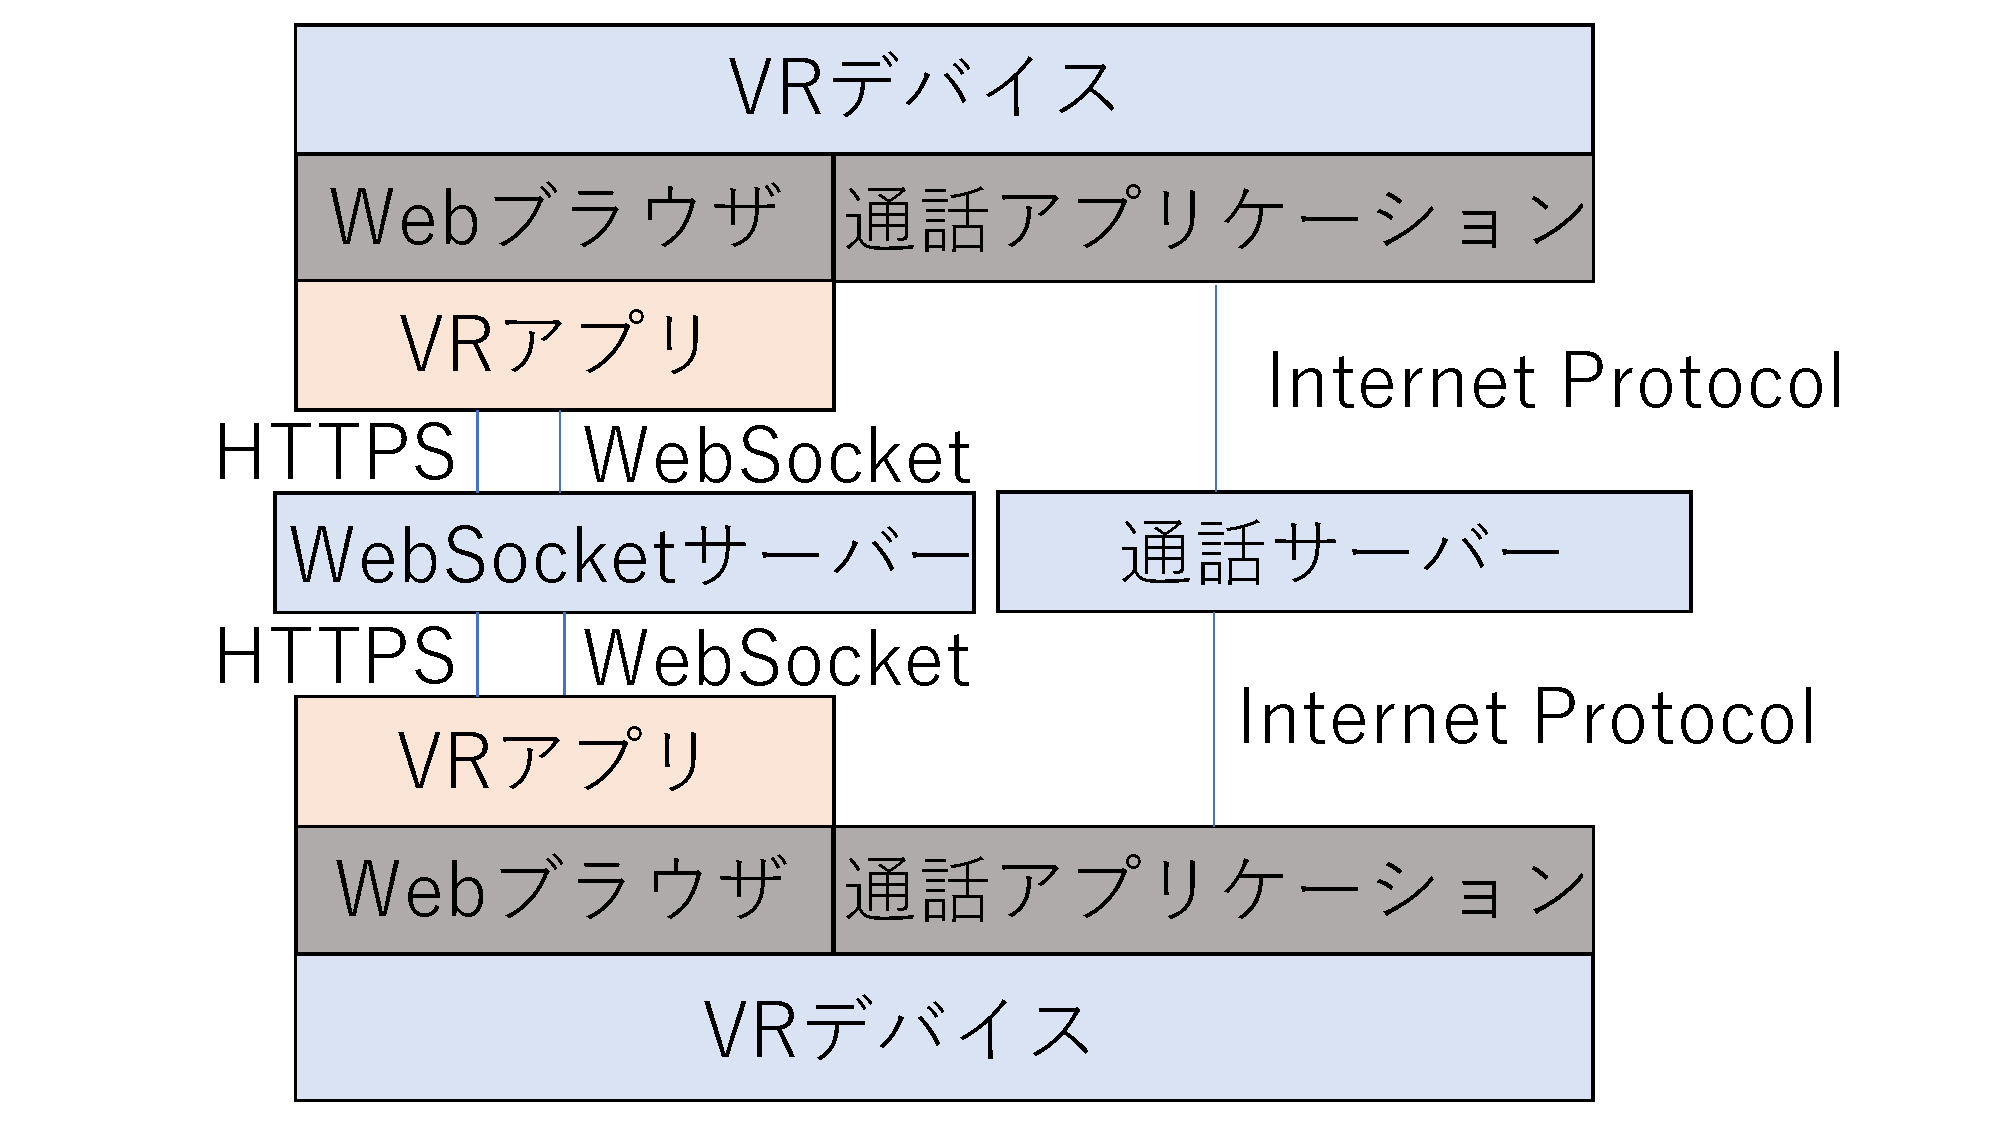
\includegraphics[width=90mm]{systemkouzou.pdf}
\end{center}
 \caption{システム構成図}
 \label{fig:system}
\end{figure}

\section{おわりに}
本研究ではデートに対する不安を軽減するアプリを開発した.今後は実際に利用してもらい,どの程度恐怖や不安が軽減されたのか調査していきたい.

\begin{thebibliography}{99}
\bibitem{naikakufu2019} 内閣府: ``少子化対策の現状'', \url{https://www8.cao.go.jp/shoushi/shoushika/whitepaper/measures/w-2016/28webhonpen/html/b1_s1-1-3.html}, 2019/3/26参照
\bibitem{prtimes}PRTIMES:``マッチングアプリは怖い?危ない目に合った?初めて会うまでの期間は!?徹底調査'',
\url{https://prtimes.jp/main/html/rd/p/000000016.000059676.html},2021/10/4参照
\bibitem{yoshimura2020} 古村 健太郎: ``成人のマッチングアプリ利用の背景-成人のマッチングアプリ利用に関する研究'', 「日本心理学会大会発表論文」,第84号,pc-006(2020)

\end{thebibliography}


\end{document}
